\documentclass{article}
\usepackage[screen]{geometry}
\usepackage{alltt,xcolor}
\usepackage[utf8]{inputenc}
\usepackage{listings}
\usepackage{graphicx}
\lstset{escapechar=\@,language=C++,keywordstyle=\color{blue},showstringspaces=false}
\begin{document}
\large
\section*{Specification}
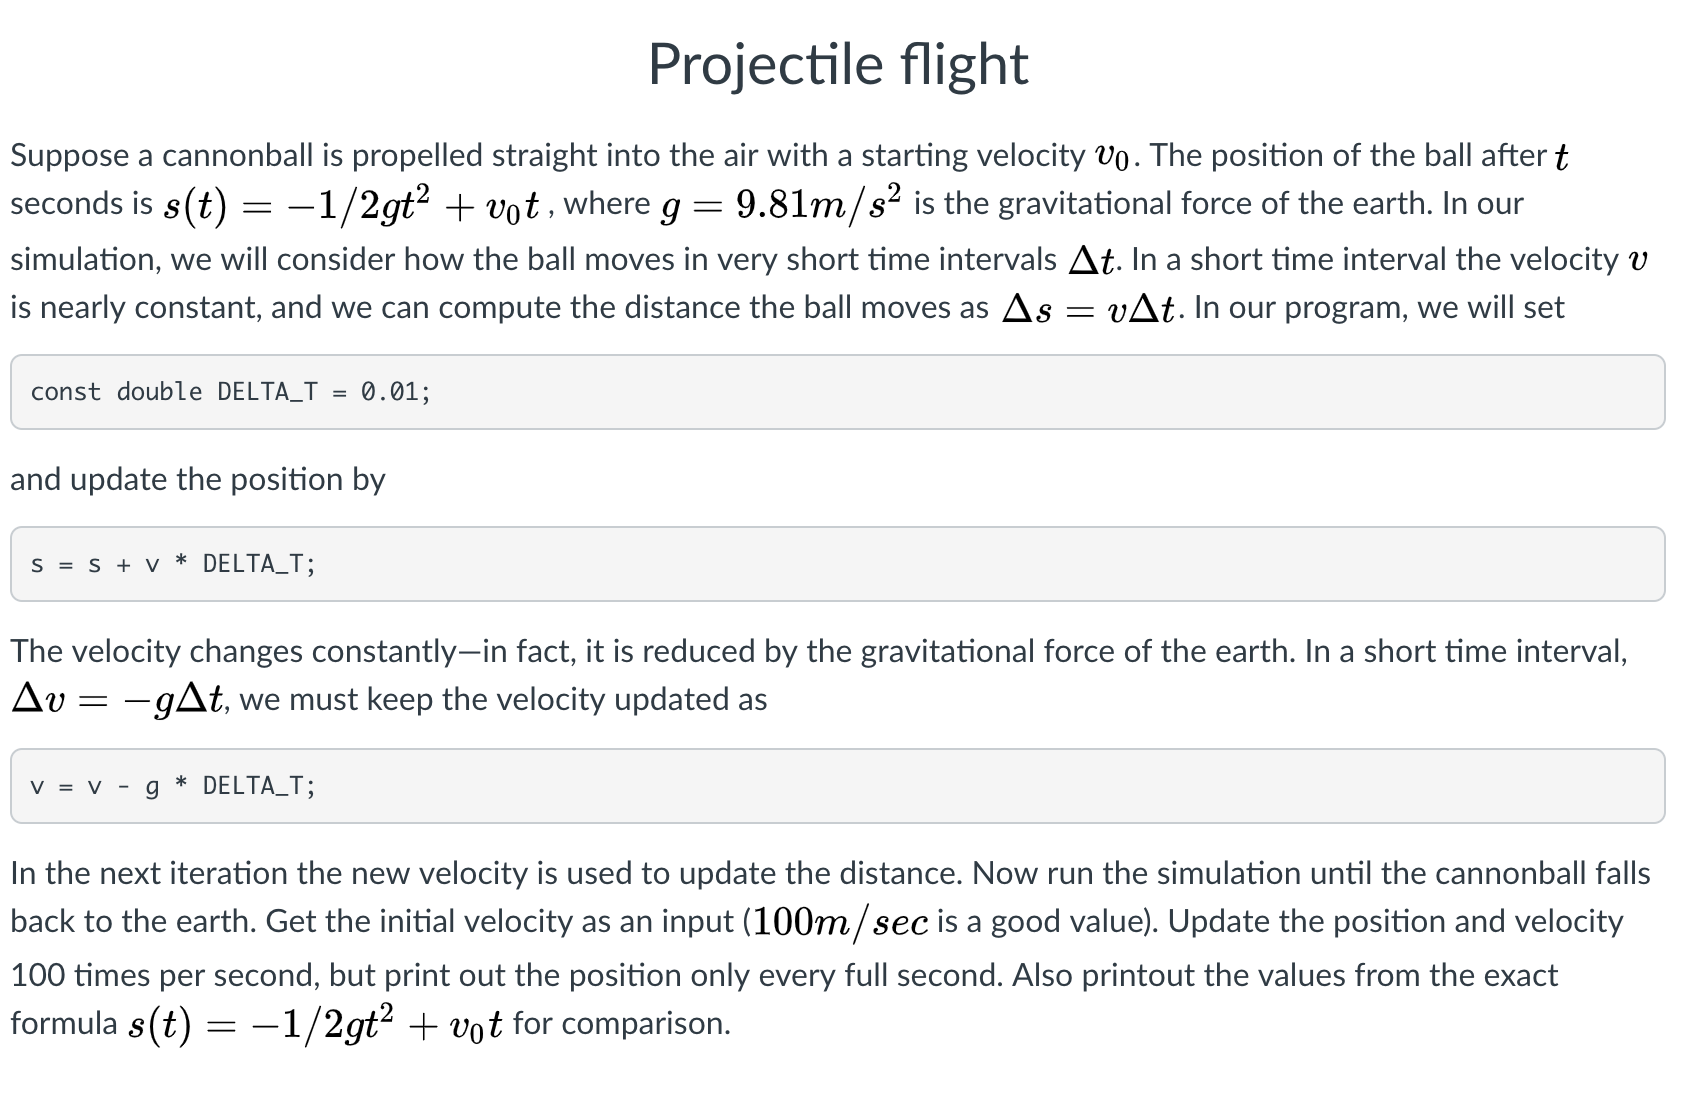
\includegraphics[width = 19cm, height = 11cm]{part1.png}
\newpage
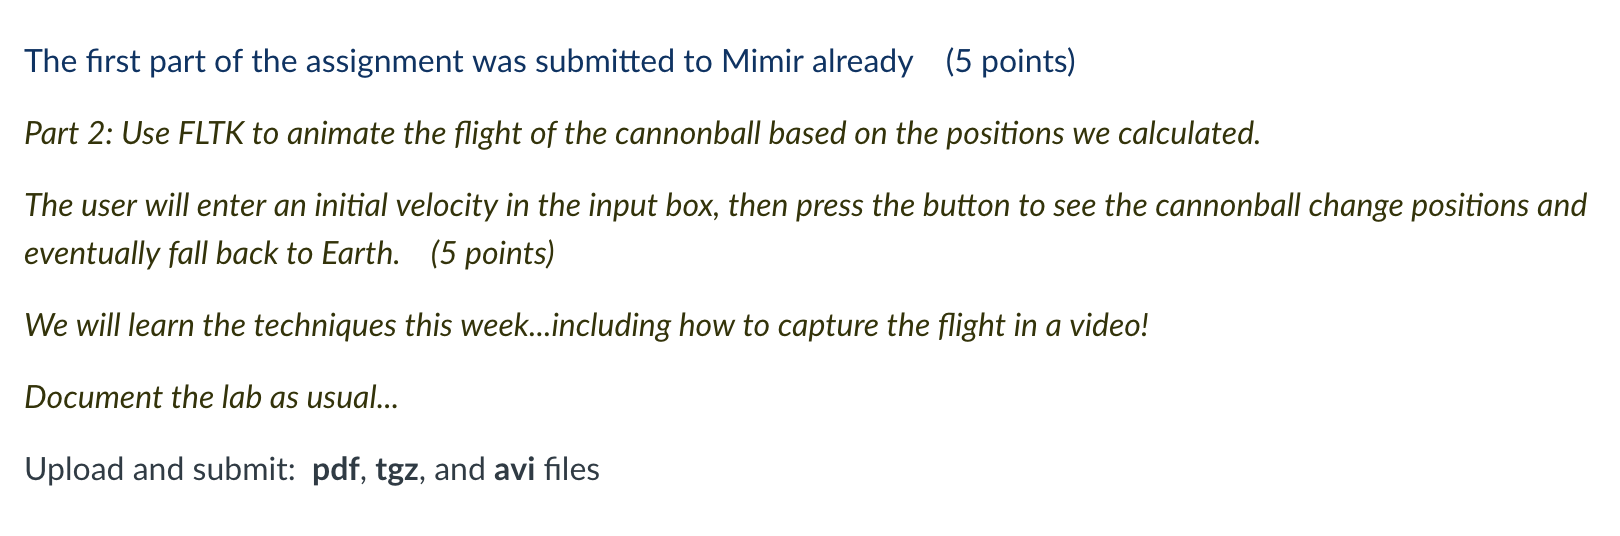
\includegraphics[width = 19cm, height = 6cm]{part2.png}
\newpage\section*{Analysis}
\begin{description}
	\item [Inputs]  The initial volecity $v_{0},\Delta t = 0.01, g = 9.81$
	\item [Process]  Calculate the distance s (position of the cannonball) from input $v_{0},v$,and update it.
	where at the first time,$v=v_{0}$and then we can enter the loop where $ v=v-g*\Delta t , s=s+v*\Delta t$ will be process every 0.01 second.
	\item (And at the same time,we need to use fltk to make a window where the user will enter an initial velocity in the input box, then press the button to see the cannonball change positions and eventually fall back to Earth.)
    \item [Outputs]  The distance will be translated into the position of the ball by using the functions representing width and height as  x and y in coordinate system.That's how we get our output.
\end{description}
\newpage\section*{Design}
\begin{enumerate}
	\item Define constants and variables
	\subitem The graviational constant is 9.81 m/sec
	\subitem v is velovity, s is position, t is time
	\subitem Delta time is constant intercal = 0.01
	\item Get initial velovity from user
	\item set v to initial velovity
	\item Display column hraders
	\item Reapte until cannonball hits the earth
	\begin{enumerate}
		\item display each row each hundredth iteration(seconds, 
		incrementslly calculated position,
		position calculated using formula)
		\subitem (because dispay seconds but time interval is  0.01 seconds)
		\item Update new position
		\item Update new velocity
	\end{enumerate}
	
\end{enumerate}
\newpage\section*{Implementation}
\lstinputlisting{lab.cpp}
\lstinputlisting{labgui.cpp}
\lstinputlisting{labgui.h}
\newpage\section*{Test}
\subsection*{Testcase (screen shoot)}
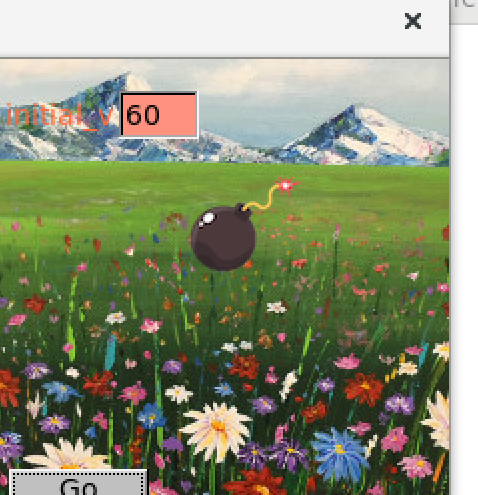
\includegraphics{te.png}
\begin{description}
	\item As we can see in the picture, my program is running successfully.The background, the bomb, and our input box appear in the corrct position.
\end{description}
\subsection*{Testcase (movie)}
\begin{description}
	\item the name of my Avi files are outputc.avi ,outputc2.avi .
	\item As we can see in the avi files, my program is running successfully.The position of the bomb update correctly, and hit the earth at last.At the same time, I have the output of the velocity and distance in the terminal , which looks nice.
\end{description}
%\includegraphics{testcase2.png}
\end{document}
